\subsection{The Backend Software Stack}
The backend software stack will be responsible for collecting data from the
sensor nodes and displaying the air quality data on webpage. It will also be
responsible for sending alerts via text or on Twitter about poor air quality
conditions. It will be the main way users will interact with their deployed
sensors and view data. The backend will also allow users to manage, configure,
and send commands to the sensor nodes remotely. The backend is composed of three
main components: (1) the LoRaWAN gateways running the LoRaWAN Network Server,
(2) a server running on an IoT host provider that can collate data from the
gateways and provide other backend services, and (3) a web user interface
running on the IoT backend provider (such as AWS IoT or Azure IoT) that displays
statistics and user specific information. Additionally, the LNS can optionally
be ran in the cloud. In this scenario, the gateway runs a LoRa packet forwarder
that understands the LNS protocol. Packets can be forwarded to the LNS data
endpoint server, and the gateway is managed through a configuration and update
server (CUPS) using the CUPS protocol along with HTTPS. While the following
software solutions offer support for LoRaWAN versions 1.0.x and 1.1, since the
chosen LoRa module only supports up to 1.0.3, the following discussions will be
with LoRaWAN 1.0.3 as there are some differences with the architecture. The
changes are in regard to the process of join the network. 

There are two types of LoRaWAN networks: public and private. Public networks are
networks akin to Verizon or AT\&T. They provide coverage and networking. Two of
the biggest LoRaWAN public networks are The Things Network and The Helium
Network. Once registered on the network, LoRaWAN devices can operate with the
developer's application server which is configured during registration. The
other option is to configure a private network. When creating a private network,
there are generally two main architectures to choose between in order to route
packets to an application server. The first option, which will be referenced as
local-LNS, is to run the entire LNS on a gateway device. This means that the
gateway needs to manage more information about the end-devices and the state of
the network. The second option, cloud-LNS, is where the gateway operates purely
as an access point, and forwards packets to a LNS in the cloud.  This offers
greater scalability and lower compute and power requirements of the gateway
device at the expense of added complexity. Luckily, there are many solutions
available through service providers, such as AWS.

\subsubsection{LoRa Packet Forwarding}
LoRa packet forwarding is the key function of a LoRaWAN gateway. As stated before, the goal of  the LoRaWAN gateway is to take data being transmitted from LoRa end-devices and route it to the internet via another communication protocol, such as WiFi. To perform this action, a LoRaWAN gateway contains a software that is referred to as the packet forwarding. This software is responsible for demodulating LoRa RF packets received from end-nodes and transmitting them to the server. 

Many different LoRa packet forwarding software exists already and can be used by anyone setting up a custom gateway. An example is the Semtech UDP Packet Forwarding. This is the original LoRa packet forwarding created by the company who created the LoRa standard. In fact, most off-the-shelf gateways include a pre-compiled version of this software. Another popular LoRa packet forwarding protocol is MQTT, which is used with Chirpstack.

\subsubsection{LoRaWAN Network Servers} The sensor nodes communicate over LoRa
using the LoRaWAN protocol to gateways.  These gateways are running what is
called the LoRaWAN Network Server (LNS), which is a standardized protocol for
connecting devices using LoRaWAN to the internet.  LoRaWAN network servers are
the bridge between LoRa and the Internet.  LoRa network servers can be public or
private, and end-devices must first be registered on the network before it can
join it. All packets sent by an unregistered and unverified end-device will be
discarded.

As previously mentioned in the LoRaWAN standardization section,
devices communicating over LoRaWAN perform a handshake (joining the network),
and exchange a set of IDs that identify the device, the join server, and the
application/network session. These IDs are: \texttt{DevEUI}, \texttt{JoinEUI} (known previously as
the \texttt{AppEUI}), and \texttt{AppKey}, respectively. The remainder of the keys are generated
from this set of keys. The \texttt{AppKey} is the only key that isn't transmitted over
the network, and is stored on both the end-device and the network server. For
LoRaWAN 1.1+, an additional key is required to be stored on the end-device and
the network server: the \texttt{NwkKey}. The \texttt{NwkKey} is like the \texttt{AppKey} in that it is
never transferred and is used as an extra encryption layer. The network server
will need to be integrated and capable of communication with the application
server, which in for the project, will either be Amazon AWS or Microsoft Azure.

For public networks, which are basically like Verizon or AT\&T for LoRa, the
network server software is provided to users who want to setup a gateway. Once
setup, anyone with reception will be able to use the network. The Things Community Stack
is a free, public network. Users that create a gateway are not financially
incentivized, but only are if they have a end-device they would like to use in
their area. On the other hand, The Helium Network provides financial incentives
without a central authority through a specialized blockchain. For people and
companies that would like to setup a private network, an open-source network
server, called Chirpstack, is available.


\paragraph{The Chirpstack Network Server Stack}

\subsubsection{Public LoRaWAN Networks} \label{public-networks}
Public LoRaWAN networks allow users to connect their own LoRa end-devices to them and begin sending data to the internet. These networks make it easier start using LoRaWAN devices and removing the need to purchase, set up, and maintain large amounts of LoRaWAN gateways. Some public networks, like The Things Community Network, are entirely free to connect to and use. However, there are others, such as The Helium Network, that take advantage of blockchain technology to charge users for the usage of the network. This functions as a way to provide a monetary incentive for users to add gateways to the network, making it larger and increasing it's coverage.

\paragraph{The Things Community Network}
The Things Community Network is a public LoRaWAN network that uses The Things Network Stack. This network was previously known as simply The Things Network. The software for this network is entirely open source, so it would be possible for someone to run their own instance of this network on their own servers. Currently, The Things Network has over 21,000 gateways in operation providing great network coverage. However, the vast majority of network coverage is in Europe. In the United States, coverage is largely centered around the northeast, with some coverage in Florida.

The Things Community Network provides a tool for adding LoRaWAN devices to the network known as The Console. It is a web application which can be used to register applications, end devices or gateways, monitor network traffic, or configure network related options, among other things. When adding a device to the The Things Community Network, there are preset device profiles for mainstream, off-the-shelf devices to make set up very straightforward. Otherwise, if a user is attempting to add a custom device, they will have to manually provide their device information (\texttt{DevEUI}, \texttt{JoinEUI}, etc.). Due to the free and public nature of The Things Community Network, they specifically mention that users should take actions to limit network use, such as limiting data transmission frequency, optimizing message encoding for size, and avoiding confirmed uplink messages \cite{the-things-network}. They recommend these practices to ensure that no single user is hoarding the usage of network resources. These sort of policies and suggestions are necessary when there is no cost to use a network.

\paragraph{The Helium Network}
The Helium Network is a public LoRaWAN network that takes advantage of blockchain and cryptocurrency technology and is made up of so-called Helium Hotspots. Hotspots produce and are compensated in HNT, which is the native cryptocurrency of the Helium blockchain. The goal of the Helium blockchain is to incentivize people to set up LoRaWAN gateways to increase the coverage of the network itself.

The Helium blockchain itself is based off of a concept known as Proof of Coverage. The goal of the Proof of Coverage algorithm is to verify that Hotspots are located where they claim to be located, as well as that they are accurately reporting the area that they claim to cover. The algorithm attempts to continuously verify these details. The Proof of Coverage does this by taking advantage of the unique properties of radio frequencies. Due the fact that the strength of a radio frequency signal is inversely proportional to the square of the distance from the transmitter and the fact that radio frequencies travel at the speed of light with effectively no delay, the Helium network can use these properties to issue challenges to the Hotspots. Completing challenges is used to determine how much HNT a Hotspot is paid.

The developers provide a tool designed to assist users in registering their devices for use on the Helium Network. This tool is known as the Helium Console. Helium requires the creation of a user account. To add a device to Helium, users must either provide the \texttt{DevEUI}, \texttt{AppEUI}, and \texttt{AppKey} that came on the device or use the one auto-generated by the Console. All devices are also provided a unique identifier when connecting to the network. The Helium network supports any LoRaWAN capable device meeting the LoRaWAN v1.0.2 specification. The LoRa module we chose for our design meets this specification.

In order to discuss how to set up your own LoRaWAN gateway as a Helium Hotspot, we must first describe the different classifications of Hotspots that Helium describes. The first type is known as a Full Hotspots. Full Hotspots maintain a full copy of the HNT blochain. This class of Hotspot is able to participate in Proof of Coverage rewards and receive awards for forwarding data packets. However, in order to be classified as a Full Hotspot, the hardware vendor of the gateway must submit an approval form that is approved by the Helium Community and the Decentralized Wireless Alliance (DeWi). The second type of Hotspot is known as a Light Hotspot. Light Hotspots use Validators to get information about the HNT blockchain. This class of Hotspot is able to participate in Proof of Coverage rewards and receive awards for forwarding data packets. The final type of Hotspot is known as a Data Only Hotpsot. These Hotspots can only receive HNT through participating in data packet forwarding. There is no community permission required to add a Data Only Hotspot to the Helium Network. A summary of these Hotspot types can be found in Table \ref{tab:helium-hotspot-classes}.

It is important to note that there is an additional entity that is a part of the Helium Network, but it is not a Hotspot. It is known as a Validator. A consensus group of Validator nodes receive Proof of Coverage and device-related transaction requests from Light Hotspots and both verifies these requests and reaches an agreement on the ordering before forming a new block and adding it to the blockchain.

\begin{table}
\centering
\caption{Summary of Helium Hotspot types}
\begin{tabular}{|l|l|l|l|}
\hline
Rewards Type & Data Only Hotspots & Full Hotspots & Light Hotspots \\
\hline\hline
Network Data Forwarding & Yes & Yes & Yes \\\hline
Proof of Coverage & No & Yes & Yes \\\hline
\end{tabular}
\label{tab:helium-hotspot-classes}
\end{table}

\subsubsection{Application Service Providers}
In this section we will describe two of the major competitors in the cloud hosting business, Amazon's AWS and Microsoft Azure. We will use the infrastructure from one of these two companies to host the software that will manage the data received from LoRaWAN gateways as well as to host the web-based user interface that will display statistics and information related to data collected from the sensor nodes. It should be noted that while we could explore the option where we perform our own hosting, the required initial monetary and time investment is far too great for our needs. This is in addition to the fact that both of these cloud service providers have free usage pricing tiers that include a feature set that is more than enough to meet our requirements.

\begin{table}[t]
\centering\footnotesize
\caption{Microsoft Azure pricing structure}
\begin{tabular}{|l|l|l|l|}
\hline
Pricing Tier & Standard Tier 0 & Standard Tier 1 & Standard Tier 2 \\
\hline\hline
Price per device per month & \$0.08 per Month & \$0.40 per Month & \$0.70 per Month \\\hline
Monthly device message allocation & 400 messages & 5,000 messages & 30,000 messages \\\hline
Included free quantities per application & 2 free devices & 2 free devices  & 2 free devices  \\\hline
Overage pricing per 1K messages & \$0.07 & \$0.015 & \$0.015 \\\hline
\end{tabular}
\label{tab:azure-pricing}
\end{table}

\paragraph{Microsoft Azure}
Microsoft Azure is a cloud computing service that is operated by Microsoft through their own data centers. Azure is composed of large number of different services. One of those services is known as Azure IoT. This is the service that we would primarily be using for our project. Azure IoT itself is made up of a large quantity of tools and sub-services that were created to assist users of Azure IoT with building their application. These would be the features of Azure that we would need to use and interact with to build our project.

One of these tools is known as Azure IoT Central. This is a tool that allows for the rapid and easy creation of web applications due to the plug-and-play nature and large quantity of templates. This tool makes it easy to quickly setup a web application that can display data from our sensor nodes.

Another tool is known as Azure IoT Hub. The goal of this tool is to enable secure and reliable communication between an IoT web application and the devices that it manages. It is essentially a cloud-hosted backend that connects virtually any device. Azure IoT Hub also supports the ability to send device-to-cloud messages. These messages allow the user to understand the state of the device and define message routes to other Azure tools and services. Azure IoT Hub also supports the ability to send cloud-to-device messages. These messages allow the user to reliably send commands and notifications to any connected devices and track message delivery with acknowledgement receipts. This allows for bidirectional communication between devices and the cloud.

Besides features, another critical factor when deciding what cloud hosting service we are going to use is price. Azure IoT has three pricing tiers. As you move up in the tiers you gain access to resources, meaning you can connect more IoT devices and send more messages, however, you start to pay more per month. For our purposes, Standard Tier 0 is more than enough. We plan to connect no more than two to three devices (one or two sensor nodes and a gateway). This would mean that we stay within the "2 free devices" portion of the tier and even if we were to connect more, the price would still only be \$0.08 per additional device per month. Additionally, our design does require the transmission of that many messages per day, meaning that should stay well within the limit of 400 messages per month. The breakdown of the pricing scheme can be found in Table \ref{tab:azure-pricing}.



\paragraph{Amazon AWS}
Amazon AWS is another major cloud computing service provider, especially known
for their mature products and services, as well as consistent and dependable
uptime. Amazon owns FreeRTOS, so there is dedicated middleware support for
connecting to the cloud and using a variety of services. This includes update
over the air and digital signing service functionalities. Amazon offers
dedicated IoT services, as well as anything else to meet the needs of your
application. The entire software stack, ranging from IoT device management, IoT
event transactions, and IoT analytics to the SQL or NoSQL database, website
hosting, and social integration, such as Twitter, email, or SMS. AWS most
importantly has direct support for LoRaWAN IoT devices. This means that you can
run a LNS in the cloud, further securing the LoRa network. 

\begin{figure}
  \centering
  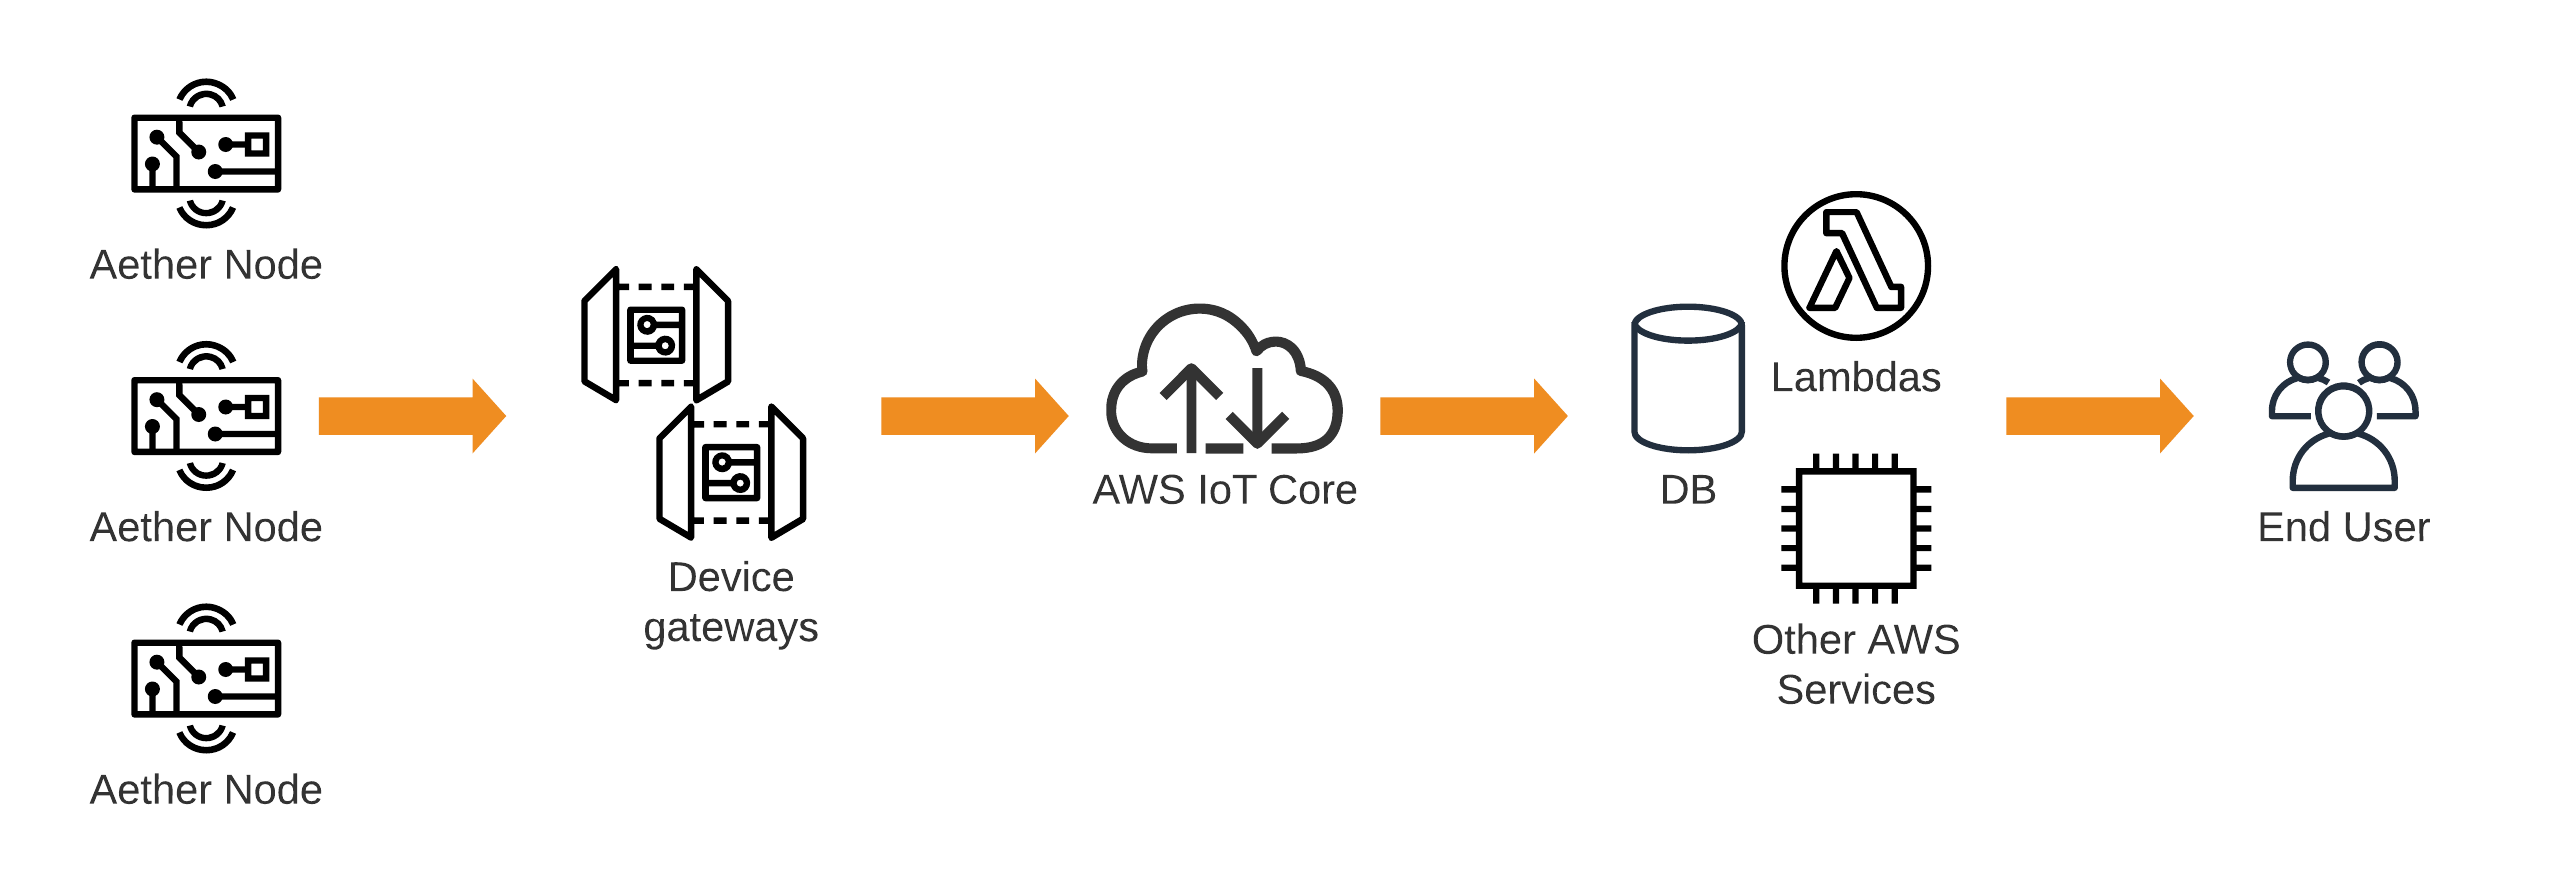
\includegraphics[width=5in]{aws-iot-core.png}
  \caption{Amazon Web Services IoT Core Network Diagram}
  \label{aws-iot-core}
\end{figure}

Because the LoRa network server doesn't have to run on the gateway, the gateway
can have lower processing requirements and the data on the network is  less
susceptible to be able to be compromised since the gateway won't be managing the
state of the network. In this scenario, the gateway would only implement a
LoRaWAN packet forward, otherwise known as a \emph{bridge}, to purely translate
packets between LoRaWAN and the internet protocol (IP), and forward them to the
LNS running in the AWS cloud. AWS' IoT Core allows the LNS service to integrate
with the rest of an application's services through the MQTT protocol. MQTT
stands for "Message Queuing Telemetry Transport", and it is a protocol built
for IoT devices to provide an easier-to-use, light-weight publish/subscribe
message transport protocol to take place of HTTP/HTTPS. It's perfect for
resource-limited IoT devices where mainly all they need to do is inform a server
of some event that happened. The MQTT protocol runs on top of the TCP/IP
protocol. The IoT core also provides AWS Lambda execution, which are quick start
up, server-less, and reactive compute service that automatically scales based on
need. Lambdas, and other forms of server processing, can be triggered based on
event rules. Rules are filters and binning services that allow an application to
trigger events and/or run certain functions when an IoT message matching a
rule-set is received. Rules can be created to filter messages based on device,
node types, device groups, or any other field in MQTT messages.


Through AWS' IoT device management service, devices can be registered in bulk.
It also allows users the ability to organize, track, and manage their devices
depending on their business and security needs. Through the manager, firmware
upgrades can be dispatched, and automatically manage which specific devices need
to be updated. Commands can be operated on fleets of devices, and allow for
secure remote execution. The IoT device manager has integration with many of
Amazon's other IoT specific and non-IoT services to provide a cohesive
experience for the developer, and speed users expect.

% Add final price table for AWS

% Add paragraph describing why we went with AWS

\subsubsection{The Web Application Software Stack}
The front facing user web application will be the main way of interfacing and
managing the nodes, as well as viewing the measured data in a visual and
graphical format. The application will need to allow the user to login, and
manage their own nodes. They should also be able to remotely control them, view
analytics, such as the time last seen, its approximate location, and the
individual packets. The user should also be able to configure notification
settings. The notification types will be email, SMS, and Twitter, which will all
be provided by Amazon's Simple Notification Service (SNS), as shown in Figure
\ref{server-stack}. The website will be hosted through the AWS Amplify service,
and the API endpoints to interface with the backend to retrieve sensor data,
device configuration, and other important pieces of information and
configuration will be implemented through the AWS API Gateway service. These two
services make up the "Web Server and Backend Interface" layer in the figure. The
"Application Supporting Services" layer is composed of services that help bridge
the gap between the IoT layers and the web app layers. The Amazon DynamoDB is a
NoSQL database, and is where the API gateway, AWS Lambda, and AWS IoT Events
will share data. The Amazon Cognito user authentication is for logging in users
in securely. 

AWS IoT Events provides a rule making service for identifying and
notifying of extenuating circumstances from data received from IoT devices on
the network. This service will be utilized to help create the email, SMS, and/or
Twitter alerts as previously mentioned. Events and rules, just like the rule
engine in the IoT Core service, use an SQL-like language to specify how to read
data and how to act on it. The difference between IoT Events and the IoT rule
engine is that IoT Events can be used for identifying issues for groups of IoT
devices, and is continuously monitoring devices for failures, or other special
case. The IoT rule engine, however, is for routing incoming MQTT messages to AWS
Lambda, or other services to be further processed. IoT Events can also integrate
with AWS Lambda and other services, but its use cases are entirely different.
AWS Lambda is a server-less computing engine service. In computing, lambdas are
functions that can be passed around like variables, and can be created at
runtime.

AWS Lambda allows the developer to write functions that can be
instantiated, and automatically previsioned in the cloud, whenever an event or
other service requests one. For example, AWS Lambdas could be used to decode
binary MQTT messages into JSON, or another human readable format. The web
server, AWS Amplify, could also request Lambdas to be execute, not just the Iot
core. The last layer in the backend stack is the "LoRaWAN Network Server, MQTT
Broker, IoT Services" layer. Here, the LoRaWAN Network Server is run, along with
services to accept and send MQTT messages, manage devices, and route MQTT
messages to other services. This is the layer that the LoRaWAN gateway packet
forwarder will directly talk to.

As for the web front-end, the React Javascript framework will be utilized with Typescript to quickly and more easily catch errors before deployment. React is a component-based Javascript framework originally developed by Facebook. It provides a virtual DOM (document object model), so that only specific parts of a web page are updated when the data behind them do. This is unlike how some traditional Javascript-only, DOM-driven websites were developed previously. Without a virtual DOM, it's impossible to safely know how changing data might affect the whole page, so the whole DOM was updated every time the state changed. React has a plentiful ecosystem of plugins, additional libraries, and tons of additonal documentation and help online from the huge community it has garnered.


\begin{figure}
  \centering
  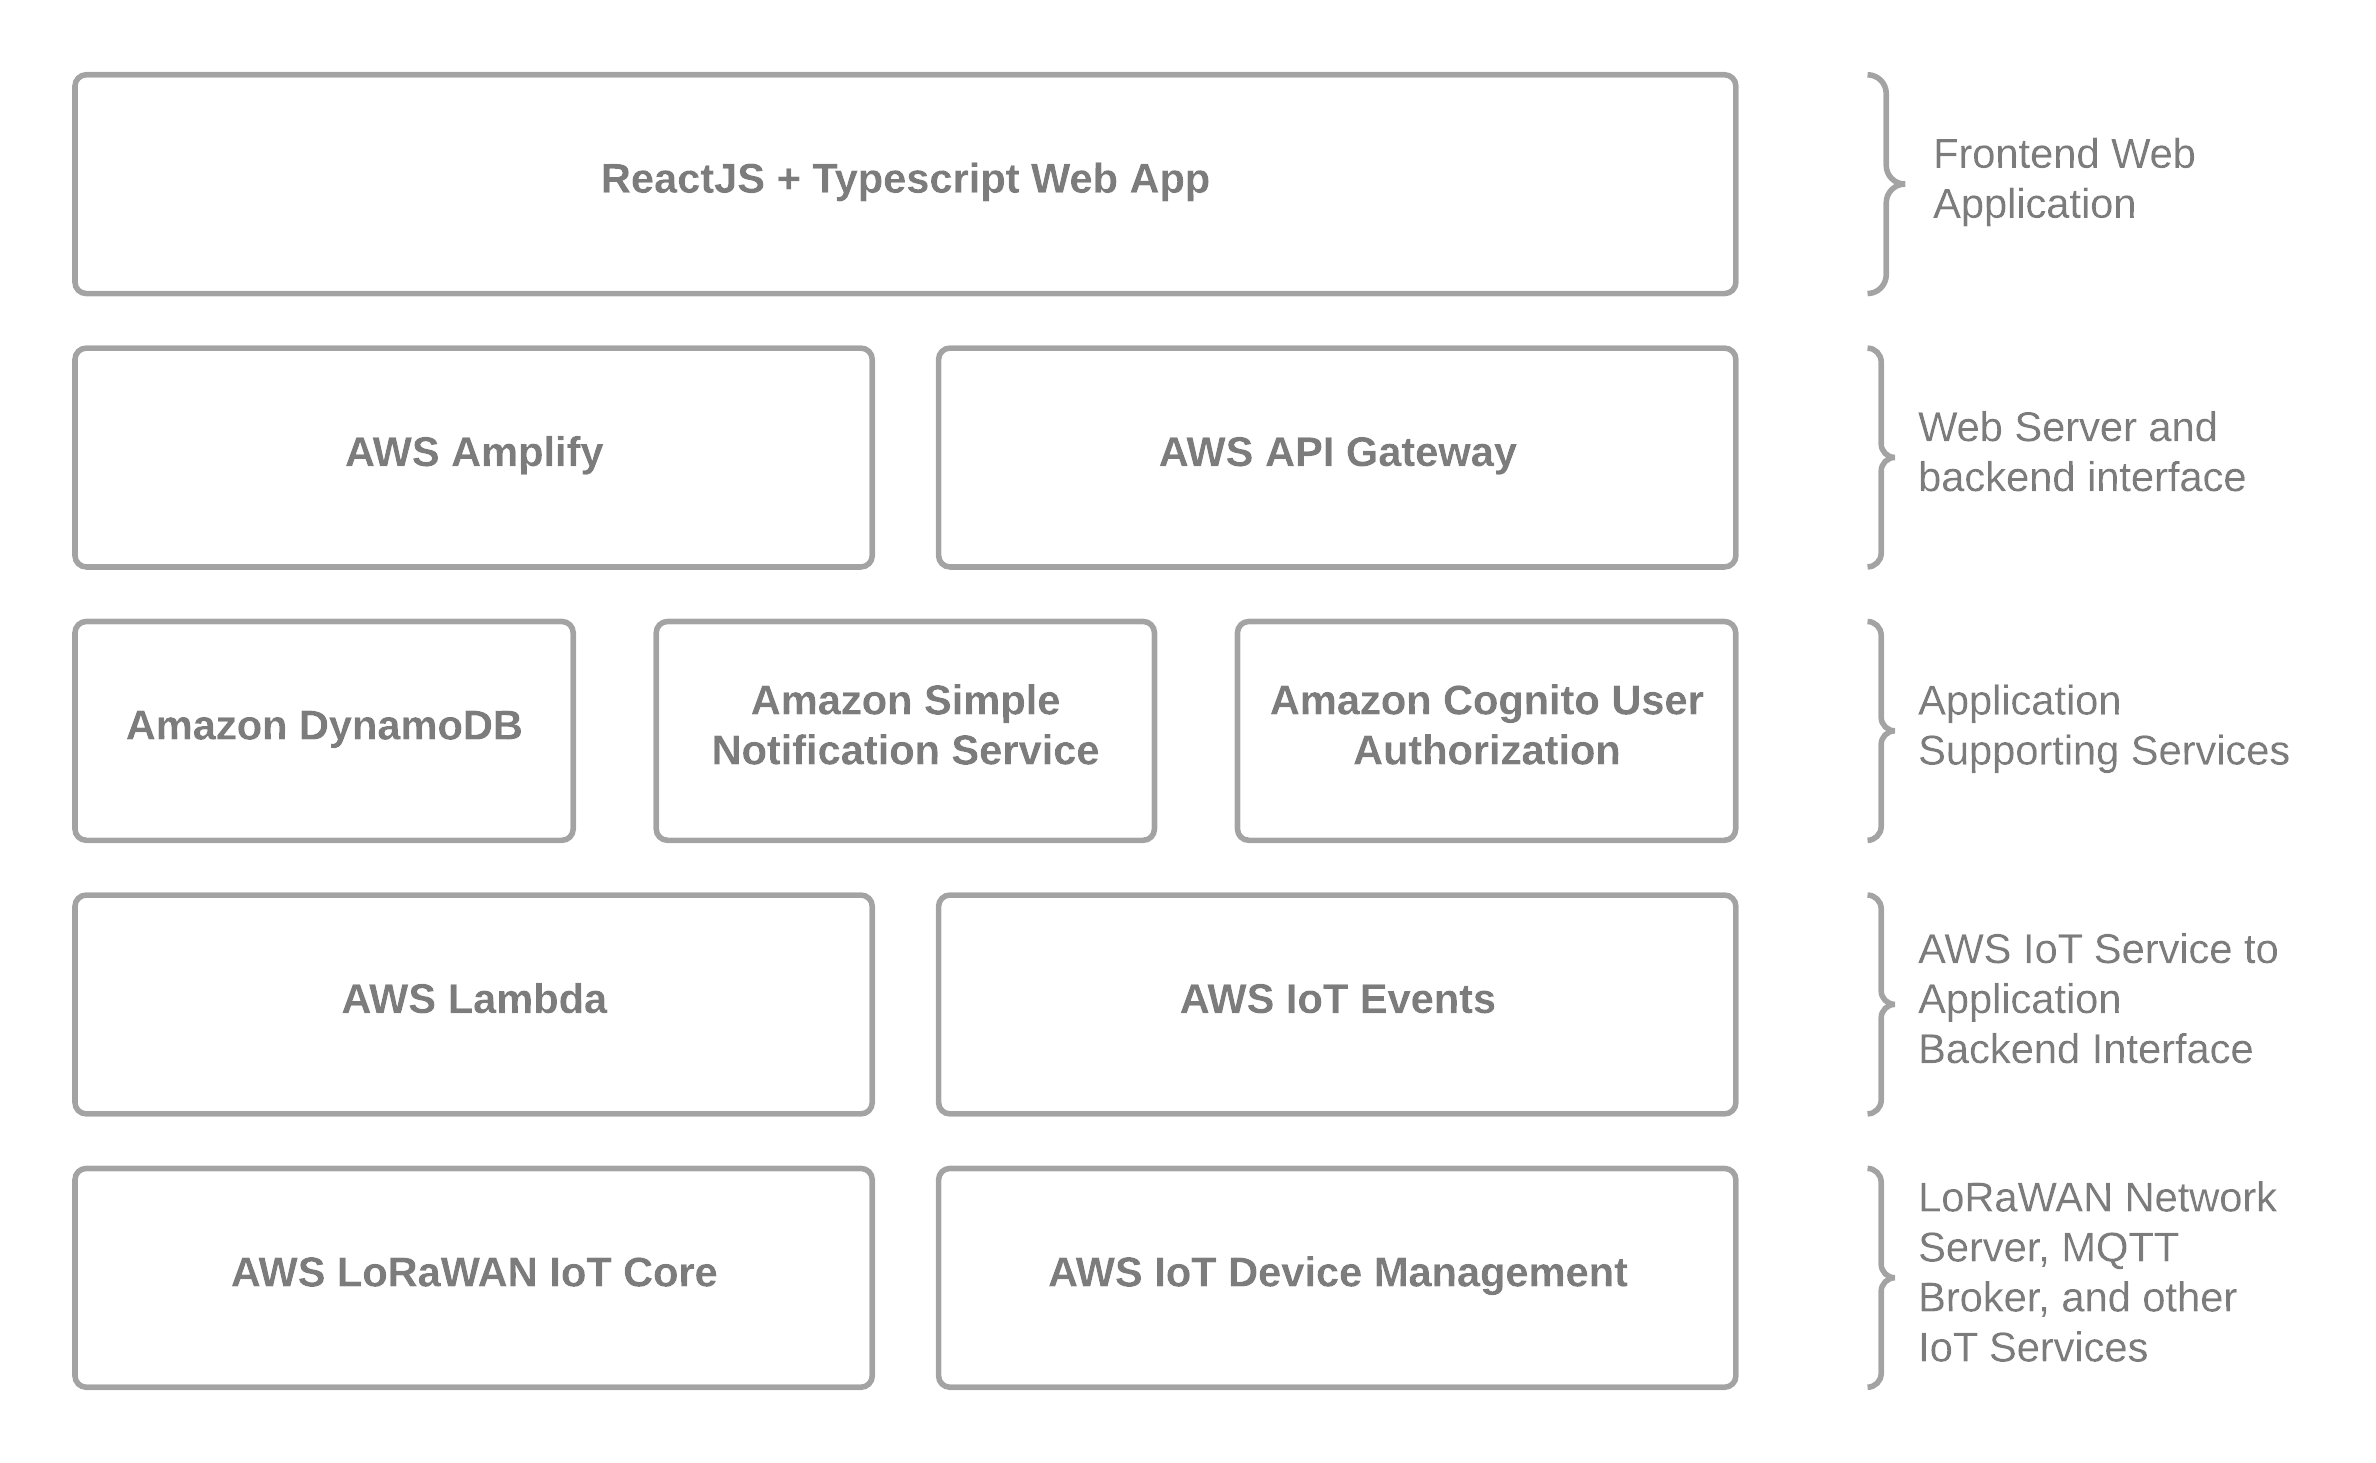
\includegraphics[width=5in]{server-stack}
  \caption{Backend Server and Web Application Stack}
  \label{server-stack}
\end{figure}

\begin{table}[H]
\centering\scriptsize
\caption{Amazon Web Services Pricing Estimate}
\begin{tabular}{|r|c|c|}
\hline
Service & Use & Price (\$)\\
\hline\hline

AWS LoRaWAN IoT Core & LoRa NS & \\\hline
AWS IoT Device Management & & \\\hline
AWS Lambda & & \\\hline
AWS IoT Events & & \\\hline
Amazon DynamoDB & & \\\hline
Amazon SNS & & \\\hline
Amazon Cognito & & \\\hline
AWS Amplify & & \\\hline
AWS API Gateway & & \\\hline

\end{tabular}
\label{lora-module-io}
\end{table}